\documentclass{beamer}
\mode<presentation> {
\usepackage{color}
\definecolor{bottomcolour}{rgb}{0.21,0.11,0.21}
\definecolor{middlecolour}{rgb}{0.21,0.11,0.21}
\setbeamercolor{structure}{fg=white}
\setbeamertemplate{frametitle}[default]%[center]
\setbeamercolor{normal text}{bg=black, fg=white}
\setbeamertemplate{background canvas}[vertical shading]
[bottom=bottomcolour, middle=middlecolour, top=black]
\setbeamertemplate{items}[circle]
\setbeamertemplate{navigation symbols}{} %no nav symbols
\setbeamercolor{block title}{use=structure,fg=white,bg=structure.fg!50!red!50!blue!100!green}
\setbeamercolor{block body}{parent=normal text,use=block title,bg=block title.bg!5!white!10!bg,fg=white}
\setbeamertemplate{navigation symbols}{}
\newcounter{moncompteur}
}
\usepackage{graphicx} 
\usepackage{booktabs} 
\usepackage[utf8]{inputenc}  
\usepackage{geometry}     
%\usepackage[francais]{babel} 
\usepackage{eurosym}
\usepackage{verbatim}
\usepackage{ragged2e}
\justifying
%%%%%%%%%%%%%%%%%%%%%%%%%%%%%%%%%%%%%%%%%%%%%%%%%%%%%%%%%%%%%%%%
%% ccBeamer 0.1, 2007-07-02                                   %%
%% Written by Sebastian Pipping <webmaster@hartwork.org>      %%
%% ---------------------------------------------------------- %%
%% Licensed under Creative Commons Attribution-ShareAlike 3.0 %%
%% http://creativecommons.org/licenses/by-sa/3.0/             %%
%%%%%%%%%%%%%%%%%%%%%%%%%%%%%%%%%%%%%%%%%%%%%%%%%%%%%%%%%%%%%%%%


%% Images
\newcommand{\CcImageBy}[1]{%
	
\includegraphics[scale=#1]{creative_commons/cc_by_30.pdf}%
}
\newcommand{\CcImageCc}[1]{%
	
\includegraphics[scale=#1]{creative_commons/cc_cc_30.pdf}%
}
\newcommand{\CcImageDevNations}[1]{%
	
\includegraphics[scale=#1]{creative_commons/cc_dev_nations_30.pdf}%
}
\newcommand{\CcImageNc}[1]{%
	
\includegraphics[scale=#1]{creative_commons/cc_nc_30.pdf}%
}
\newcommand{\CcImageNd}[1]{%
	
\includegraphics[scale=#1]{creative_commons/cc_nd_30.pdf}%
}
\newcommand{\CcImagePd}[1]{%
	
\includegraphics[scale=#1]{creative_commons/cc_pd_30.pdf}%
}
\newcommand{\CcImageSa}[1]{%
	
\includegraphics[scale=#1]{creative_commons/cc_sa_30.pdf}%
}
\newcommand{\CcImageSampling}[1]{%
	
\includegraphics[scale=#1]{creative_commons/cc_sampling_30.pdf}%
}
\newcommand{\CcImageSamplingPlus}[1]{%
	
\includegraphics[scale=#1]{creative_commons/cc_sampling_plus_30.pdf}%
}


%% Groups
\newcommand{\CcGroupBy}[1]{% zoom
	\CcImageBy{#1}%
}
\newcommand{\CcGroupByNc}[2]{% zoom, gap
	\CcImageBy{#1}\hspace*{#2}\CcImageNc{#1}%
}
\newcommand{\CcGroupByNcNd}[2]{% zoom, gap
	\CcImageBy{#1}\hspace*{#2}\CcImageNc{#1}\hspace*{#2}\CcImageNd{#1}%
}
\newcommand{\CcGroupByNcSa}[2]{% zoom, gap
	\CcImageBy{#1}\hspace*{#2}\CcImageNc{#1}\hspace*{#2}\CcImageSa{#1}%
}
\newcommand{\CcGroupByNd}[2]{% zoom, gap
	\CcImageBy{#1}\hspace*{#2}\CcImageNd{#1}%
}
\newcommand{\CcGroupBySa}[2]{% zoom, gap
	\CcImageBy{#1}\hspace*{#2}\CcImageSa{#1}%
}
\newcommand{\CcGroupDevNations}[1]{% zoom
	\CcImageDevNations{#1}%
}
\newcommand{\CcGroupNcSampling}[2]{% zoom, gap
	\CcImageNc{#1}\hspace*{#2}\CcImageSampling{#1}%
}
\newcommand{\CcGroupPd}[1]{% zoom
	\CcImagePd{#1}%
}
\newcommand{\CcGroupSampling}[1]{% zoom
	\CcImageSampling{#1}%
}
\newcommand{\CcGroupSamplingPlus}[1]{% zoom
	\CcImageSamplingPlus{#1}%
}


%% Text
\newcommand{\CcLongnameBy}{Attribution}
\newcommand{\CcLongnameByNc}{Attribution-NonCommercial}
\newcommand{\CcLongnameByNcNd}{Attribution-NoDerivs}
\newcommand{\CcLongnameByNcSa}{Attribution-NonCommercial-ShareAlike}
\newcommand{\CcLongnameByNd}{Attribution-NoDerivs}
\newcommand{\CcLongnameBySa}{Attribution-ShareAlike}

\newcommand{\CcNote}[1]{% longname
	This work is licensed under the \textit{Creative Commons #1 3.0 License}.%
}

\title[Petit guide d'hygiène numérique]{Petit guide d'hygiène numérique} 
\author{Genma}
\begin{document}
%% Titlepage
\begin{frame}
	\titlepage
	\vfill
	\begin{center}
		\CcGroupByNcSa{0.83}{0.95ex}\\[2.5ex]
		{\tiny\CcNote{\CcLongnameByNcSa}}
		\vspace*{-2.5ex}
	\end{center}
\end{frame}
%----------------------------------------------------------------------------------------
\begin{frame}
\frametitle{L'hygiène numérique?}
\begin{block}{}
\justifying{
L'hygiène est un ensemble de mesures destinées à prévenir les infections et l'apparition de maladies infectieuses.
\\
Ce guide d''hygiène numérique, ce sont des règles destinées à mieux utiliser son ordinateur, en sécurité, de façon simple.
}
\end{block}
\end{frame}
%----------------------------------------------------------------------------------------
\begin{frame}
\begin{center}
\Huge{Quelques règles}
\end{center}
\end{frame}
%----------------------------------------------------------------------------------------
\begin{frame}
\frametitle{Les règles de sécurité}
\begin{center}
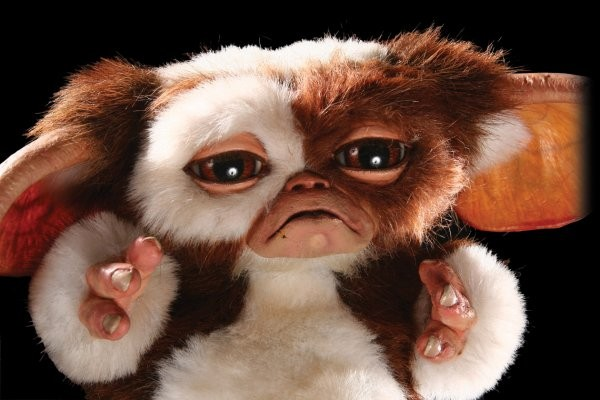
\includegraphics[scale=0.3] {./images/sadgizmo_large.jpeg}
\end{center}

\justifying{
\begin{block}{}
\begin{itemize}
\item Ne pas exposer l'animal à la lumière — et plus spécialement à celle du soleil qui le tuerait, 
\item Ne pas le mouiller, 
\item Et surtout, quoi qu'il arrive, ne jamais lui donner à manger après minuit.
\end{itemize}
\end{block}
}
\end{frame}
%----------------------------------------------------------------------------------------
\begin{frame}
\begin{center}
\Huge{Plus sérieusement}
\end{center}
\end{frame}

%----------------------------------------------------------------------------------------
\begin{frame}

\frametitle{Règle  \themoncompteur \  - Mises à jour de sécurité}
\justifying{
\begin{block}{FAIRE LES MISES A JOUR}
\begin{itemize}
\item Avoir un système à jour.
\item Avoir des logiciels à jour.
\item Avoir un antivirus à jour.
\end{itemize}
\end{block}
}

\begin{block}{Les logiciels ont des bugs}
\begin{itemize}
\justifying{
\item Un bug peut-être utilisé par un virus...
 \item Mettre à jour, c'est corriger les bugs, donc se protéger.
}\end{itemize}
\end{block}
\end{frame}

%----------------------------------------------------------------------------------------
\begin{frame}
\frametitle{Règle \themoncompteur \  - Mises à jour de sécurité}
\begin{center}
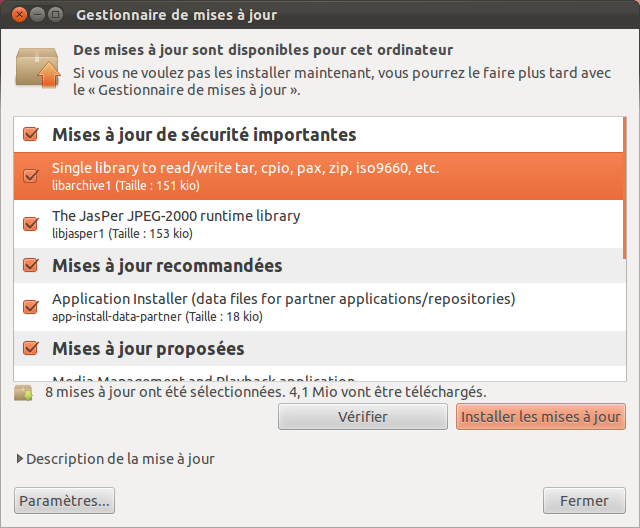
\includegraphics[scale=0.3] {./images/Maj02.png}
\end{center}
\end{frame}

\begin{frame}
\frametitle{Règle \themoncompteur \  - Mises à jour de sécurité}
\begin{center}
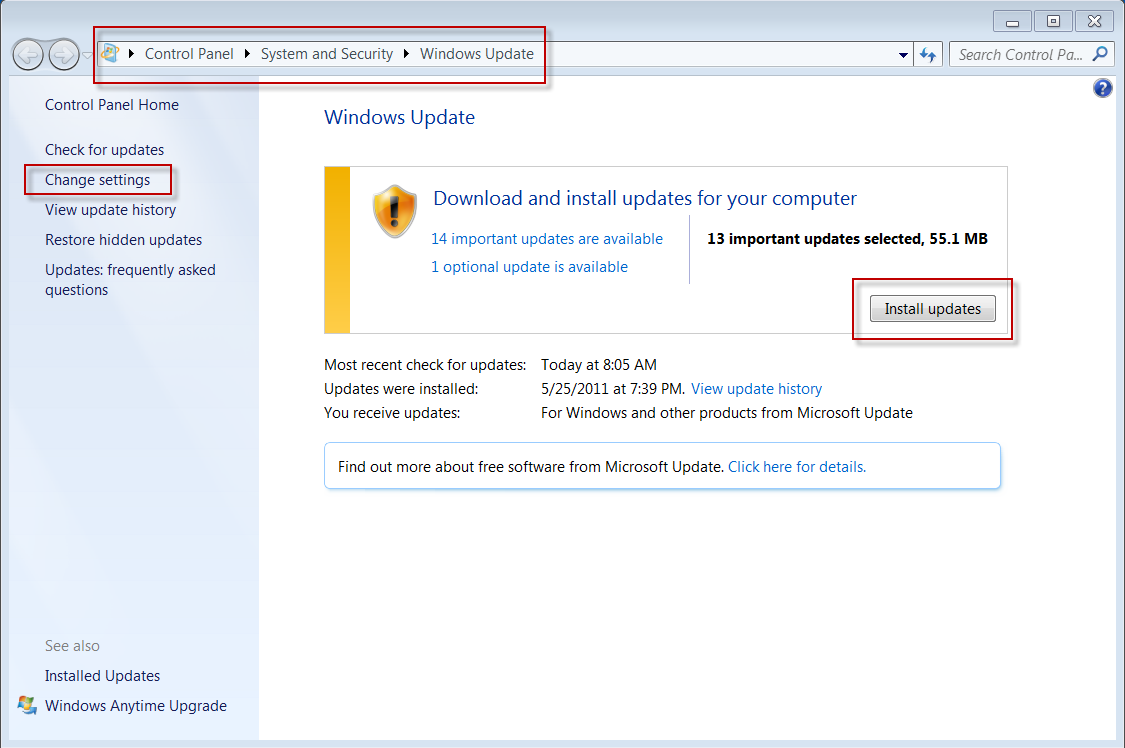
\includegraphics[scale=0.4] {./images/Maj01.png}
\end{center}
\end{frame}
\addtocounter{moncompteur}{1}

%----------------------------------------------------------------------------------------
\begin{frame}

\frametitle{Règle \themoncompteur \  - Gestion des comptes}
\begin{block}{Des comptes pour des usages différents}
\begin{itemize}
\justifying{
\item Créer un compte utilisateur et un compte administrateur.
\item Au quotidien, utiliser le compte utilisateur.
\item Le compte administrateur porte bien son nom, il ne doit servir qu'aux tâches d'administration (installation des logiciels...)
}
\end{itemize}
\justifying{
Quand l'ordinateur pose une question "Je dois lancer ce programme", réfléchir. Ne pas dire oui tout de suite.
}
\end{block}
\end{frame}
\addtocounter{moncompteur}{1}

%----------------------------------------------------------------------------------------
\begin{frame}

\frametitle{Règle \themoncompteur \  - Mots de passe}
\begin{block}{Règles}
\begin{itemize}
\justifying{
\item Plus c'est long, plus c'est bon
\item Ne pas avoir le même mot de passe pour deux comptes en lignes.
}
\end{itemize}
\end{block}

\begin{block}{Mot de passe oublié?}
\justifying{
Pour tester la sécurité d'un site web, on clique sur le lien "mot de passe oublié".
\begin{itemize}
\item Si le mot de passe est renvoyé dans le mail, ce n'est pas bon. Le mot de passe est stocké "clair".
\end{itemize}
}
\end{block}

\begin{block}{Trop de mot de passe à retenir?}
Il y a le logiciel Keepass. \url{http://www.keepass.info}
\end{block}

\end{frame}

%----------------------------------------------------------------------------------------
\begin{frame}

\frametitle{Règle \themoncompteur \  - Mots de passe}
\begin{block}{Les sites permettant de tester ses mots de passes?}
\begin{itemize}
\justifying{
\item Ils sont la meilleure façon de constituer une base de données de mots de passe.
\item Ne pas tester son vrai mot de passe mais un mot de passe du même type/de la même forme.
\item Les mots de passe sont personnels 
}
\end{itemize}
\end{block}

\begin{block}{Parents - enfants}
Tant qu’on est mineur on doit les donner à ses parents. Les parents qui sont des gens bien et responsables, ne sont pas là pour les utiliser pour espionner leurs enfants mais seulement au cas où.
\end{block}

\end{frame}
\addtocounter{moncompteur}{1}

%----------------------------------------------------------------------------------------
\begin{frame}

\frametitle{Règle \themoncompteur \  -  Les mails}

\begin{block}{Phishing - Hameçonnage}
\begin{itemize}
\justifying{
\item Ne JAMAIS envoyer d'argent. Même à un ami.
\item Etes vous sûr que c'est bien votre banque?
}
\end{itemize}
\end{block}

\begin{center}
\textbf{Toujours lire et réfléchir avant de cliquer.}
\end{center}
\end{frame}
\addtocounter{moncompteur}{1}

%----------------------------------------------------------------------------------------
\begin{frame}
\frametitle{Règle \themoncompteur \  - Le navigateur}
\justifying{
\begin{block}{Utiliser Firefox}
\begin{itemize}
\item Firefox doît être à jour.
\item Les plugins (Flash, Java) doivent être à jour.
\item Les extensions doivent être à jour.
\item Supprimer les plugins inutiles.
\end{itemize}
\end{block}
}
\begin{center}
\includegraphics[scale=0.2] {./images/Firefox.jpg}
\end{center}
\end{frame}
\addtocounter{moncompteur}{1}

\begin{frame}
\frametitle{Règle \themoncompteur \  - Les plugins}
\begin{center}
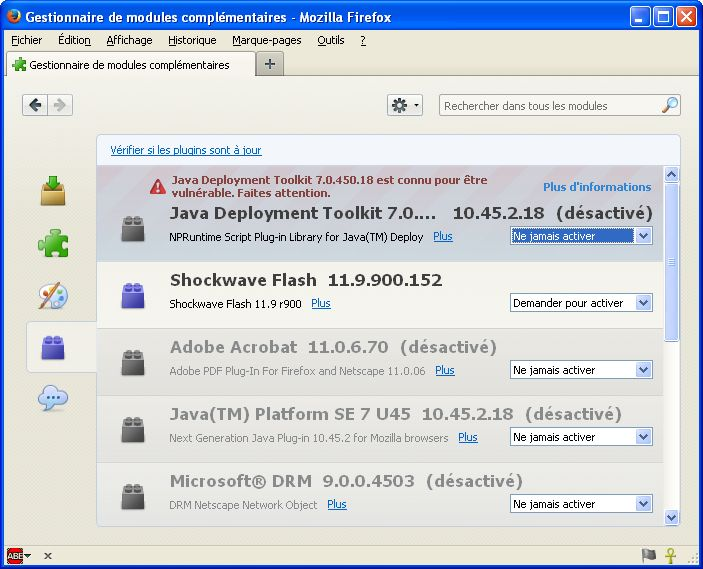
\includegraphics[scale=0.5] {./images/PluginPasAjour.jpg}
\end{center}
\end{frame}

\addtocounter{moncompteur}{1}

%----------------------------------------------------------------------------------------
\begin{frame}

\frametitle{Règle \themoncompteur \  -  Installation de logiciels}
\justifying{
\begin{block}{Logiciels payants - propriétaires}
\begin{itemize}
\item Pas de logiciels crackés
\item Pas de téléchargement de logiciels depuis un autre site que le site officiel.
On oublie les sites 01Net, Télécharger.com
\item Que les logiciels dont on a besoin (pas de démos, de logiciels marrants...)
\end{itemize}
\end{block}

\begin{block}{Logiciels libres}
\begin{itemize}
\item Préférer le logiciel libre - open-source.
\item Passer par l'annuaire de Framasoft.
\end{itemize}
\end{block}
}
\end{frame}
\addtocounter{moncompteur}{1}

%----------------------------------------------------------------------------------------
\begin{frame}
\frametitle{Règle \themoncompteur \  - Le copain qui s'y connait}

\begin{block}{Attention}
\begin{itemize}
\justifying{
\item Ne pas le laisser installer les logiciels crackés.
\item Chercher à comprendre ce qu'il fait, lui demander. 
\item S'il n'est pas capable d'expliquer, se méfier. Voire refuser.
}
\end{itemize}
\end{block}

\begin{block}{PC = Personal Computer}
\begin{itemize}
\justifying{
\item Ne pas faire confiance. Il ne faut prêter sa machine sans voir ce que fait l’individu à qui vous l’avez confié.
\item Il faut prévoir  une session invitée. 
\item Il est si facile d’installer un virus sur un PC... Méfiez-vous de ce que l'on fait sur votre PC.
}
\end{itemize}
\end{block}
\end{frame}
\addtocounter{moncompteur}{1}

%----------------------------------------------------------------------------------------
\begin{frame}
\frametitle{Règle \themoncompteur \  - Résumé}

\begin{block}{Bilan}
\begin{itemize}
\justifying{
\item Vous voulez éviter le gros de la contamination virale : Linux. 
\item Evitez les sites de Warez, de porno, les installations de logiciels piochés à gauche et à droite sur la toile, les clés USB.
\item De façon générale, lisez, apprenez, documentez vous, ayez une utilisation rationnelle de votre ordinateur. 
\item Enfin le cas échéant, quelques outils comme Malwarebytes antimalware ou Adwcleaner sont efficaces pour vérifier si la machine est saine.
 }
\end{itemize}
\end{block}
\end{frame}
\addtocounter{moncompteur}{1}

%----------------------------------------------------------------------------------------
\begin{frame}
\begin{center}
\Huge{En applicant, ces règles, on a tout de suite beaucoup moins de soucis avec son PC.}
\end{center}
\end{frame}

%----------------------------------------------------------------------------------------
\begin{frame}
\begin{center}
\Huge{En applicant, ces règles, on a tout de suite beaucoup moins de soucis avec son PC.}
\end{center}
\end{frame}
%----------------------------------------------------------------------------------------
\begin{frame}
\begin{center}
\Huge{Les sauvegardes}
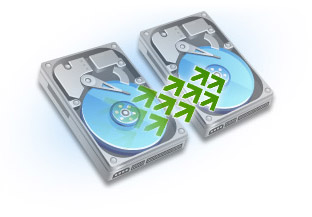
\includegraphics[scale=0.5] {./images/backup.jpg}
\end{center}
\end{frame}

%----------------------------------------------------------------------------------------
\begin{frame}
\begin{center}
\Huge{Mon PC ne marche plus, on me le vole...
Quelles sont les données que je perds?
Quelle importance ont ces données pour moi?
}

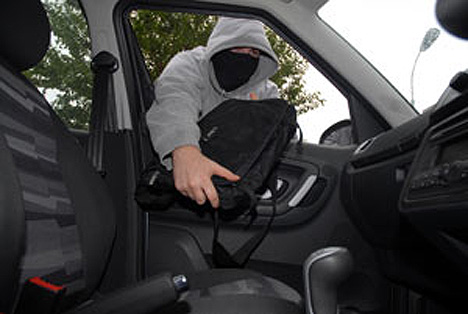
\includegraphics[scale=0.5] {./images/laptopthief.jpg}
\end{center}
\end{frame}

%----------------------------------------------------------------------------------------
\begin{frame}
\frametitle{Notre vie numérique}

\begin{block}{De plus en plus de données sont sur nos ordinateurs}
\begin{itemize}
\justifying{
\item Les photos de vacances,
\item Les factures...
}
\end{itemize}
Comment les préserver?
\end{block}
\end{frame}

%----------------------------------------------------------------------------------------
\begin{frame}
\frametitle{Sauvegarde simple et efficace}

\begin{block}{Le disque dur externe}
\begin{itemize}
\justifying{
\item Méthode simple : copier-coller.
\item Méthode plus avancé : on "synchronise".
\item On le dépose chez un ami, un voisin, un parent (pour éviter le vol, l'incendie...)
}
\end{itemize}
Petit plus : chiffrer le disque pour plus de confidentialité.
\end{block}
\begin{center}
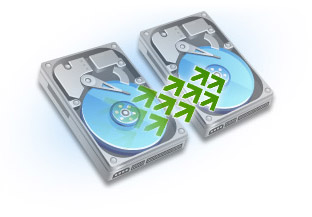
\includegraphics[scale=0.5] {./images/backup.jpg}
\end{center}

\end{frame}

%----------------------------------------------------------------------------------------
\begin{frame}
\frametitle{Sauvegarder dans le cloud?}

\begin{block}{Pratique mais...}
\begin{itemize}
\justifying{
\item Quid de la pérénité des données?
\item De la confidentialité des données?
}
\end{itemize}
\end{block}

\begin{center}
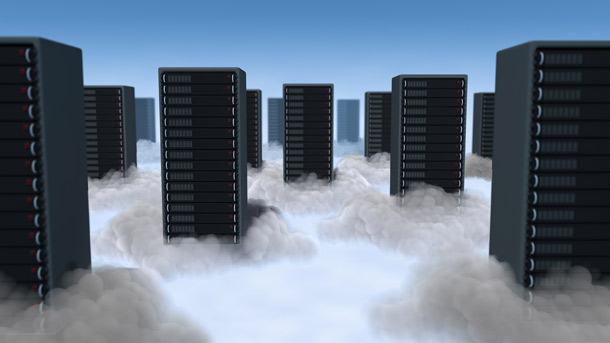
\includegraphics[scale=0.4] {./images/cloud_data_center.jpg}
\end{center}

\end{frame}

%----------------------------------------------------------------------------------------
\begin{frame}
\begin{center}
\Huge{Utilisation d'Internet \\depuis un lieu public}
\end{center}
\end{frame}


 %----------------------------------------------------------------------------------------
\begin{frame}
\frametitle{Utilisation d'un PC d'un Cybercafé?}

\begin{block}{Pour le surf Internet}
\begin{itemize}
\justifying{
\item Eviter les sites sur lesquels on sait des données personnelles : webmail, réseaux sociaux
\item Vérifier la version du navigateur
\item  Ne pas mémoriser vos informations confidentielles
\item  Penser à fermer votre session
\item  Effacer vos traces de navigation
}
\end{itemize}
\end{block}
\justifying{
Ne pas brancher de clef USB (virus), ne pas récupérer de documents.
\\
Idéalement? Un navigateur en mode portable, depuis une clef USB
\\
Encore mieux : rebooter sur un live-usb/cd
}
\end{frame}
%----------------------------------------------------------------------------------------
\begin{frame}
\frametitle{Wi-Fi public?}
Ne pas avoir confiance. Utiliser sa propre machine.
\begin{block}{Attention à la sécurisation}
\begin{itemize}
\justifying{
\item Au minimum : connexion HTTPS
\item Mieux, passer par un VPN
}
\end{itemize}
\end{block}
\end{frame}

%----------------------------------------------------------------------------------------
\begin{frame}
\frametitle{La Navigation privée}

\justifying{Naviguer sur Internet sans conserver d'informations sur les sites que vous visitez. Avertissement :
 La navigation privée n'a pas pour effet de vous rendre anonyme sur Internet. Votre fournisseur d'accès Internet, votre employeur ou les sites eux-mêmes peuvent toujours pister les pages que vous visitez.}

\begin{block}{Quelles données ne sont pas enregistrées durant la navigation privée ?}
\begin{itemize}
\justifying{
\item Pages visitées 
\item Saisies dans les formulaires et la barre de recherche
\item Mots de passe
\item Liste des téléchargements 
\item Cookies
\item Fichiers temporaires ou tampons 
}
\end{itemize}
\end{block}
\end{frame}

%----------------------------------------------------------------------------------------
\begin{frame}
\begin{center}
\Huge{Annexes}
\end{center}
\end{frame}

%----------------------------------------------------------------------------------------
\begin{frame}
\frametitle{L'authentification forte}

\begin{block}{Différents termes, un même usage}
Double authentification, Connexion en deux étapes, 2-Step Verification
\end{block}

\begin{block}{Exemple avec Google} 
\justifying{
Google permet aux utilisateurs d'utiliser un processus de vérification en deux étapes.
\begin{itemize}
\item La première étape consiste à se connecter en utilisant le nom d'utilisateur et mot de passe. Il s'agit d'une application du facteur de connaissance.
\item Au moment de la connexion Google envoit par SMS un nouveau code unique. Ce nombre doit être entré pour compléter le processus de connexion. 
\end{itemize}
Il y a aussi une application à installer qui génère un nouveau code toutes les 30 secondes.
}
\end{block}
\end{frame}

%----------------------------------------------------------------------------------------
\begin{frame}
\frametitle{L'authentification forte}
\begin{block}{Autres services implémentant cette fonctionnalité}
\begin{itemize}
\item Web : Facebook, Twitter, Linkedin, Paypal
\item Banque : envoit d'un code par SMS
\end{itemize}
\end{block}
\end{frame}
\end{document}